V následující kapitole jsou uvedeny výsledky zpracování a analýzy dat z
analogové vesmírné mise DIANA včetně výsledků experimentů strojového učení.
Kapitola je primárně rozdělena na tři části, přičemž první
sekce~\ref{sec:vysledky_qrs} uvádí pouze srovnání QRS detektorů
(viz~\ref{subsubsec:vyberqrs}). Další část je věnována prezentaci výsledků
zpracování dat z mise, primárně ve formě grafických výstupů, jako je například
vývoj sledovaných statistických veličin během mise a v rámci baterie \gls{NPF}
testů. V této části jsou také uvedeny výsledky ze statistického modelování
využitím \gls{LMM} (viz sekce~\ref{subsec:tvorba_modelů}).

V poslední části jsou uvedeny výsledky experimentů strojového učení, které byly
realizovány využitím metody navržené v rámci této práce. Samotná metoda je
detailně popsána v sekci~\ref{sec:hybridni_detekce}. Zároveň je zde uvedeno i
srovnání navržené metody se současným stavem a její experimentální ověření na
datech z mise DIANA.

\section{Srovnání QRS detektorů}
\label{sec:vysledky_qrs}
V následující tabulce jsou prezentovány výsledky srovnání QRS detektorů. Tabulka
uvádí odhady marginálních středních hodnot vysvětlující proměnné na úrovni
faktoru \enquote{Metoda}. Střední hodnota zde představuje výši chyby detektoru.

\begin{table}[!htb]
    \small
    \centering
    \caption{Výsledky výpočtu marginálních středních hodnot QRS detektorů}
    \setlength\tabcolsep{0pt}
    \begin{threeparttable}
        \begin{tabular*}{\linewidth}{@{\extracolsep{\fill}} lccc @{}}
            \toprule
            Detektor                        & Střední hodnota & SE    & 95\% CI      \\ \midrule
            *Kalidas~\cite{kalidas2017}     & 0,016           & 0,005 & 0,007 -- 0,025 \\
            Christov~\cite{Christov2004}    & 0,025           & 0,005 & 0,015 -- 0,034 \\
            Nabian~\cite{Nabian2018}        & 0,025           & 0,005 & 0,016 -- 0,034 \\
            Rodrigues~\cite{Rodrigues2021}  & 0,029           & 0,005 & 0,019 -- 0,038 \\
            Pantompkins~\cite{Tompkins1985} & 0,038           & 0,005 & 0,029 -- 0,048 \\
            Elgendi~\cite{Elgendi2010}      & 0,058           & 0,005 & 0,049 -- 0,068 \\
            Gamboa~\cite{gamboa2008}        & 0,109           & 0,008 & 0,093 -- 0,125 \\
            \bottomrule
        \end{tabular*}
        \begin{tablenotes}
            \item [*] Označuje detektor použitý v této práci
        \end{tablenotes}
    \end{threeparttable}
    \label{tab:qrs}
\end{table}

\section{Analýza dat z mise DIANA}
\label{sec:vysledky_vizual}
Ze zpracovaných biosignálů v rámci dat z mise DIANA byly vypočteny statistické
veličiny (viz sekce~\ref{subsec:sledovane_veliciny}), jejichž průměr a
směrodatná odchylka pro začátek, prostředek a konec experimentu jsou uvedeny v
Tabulce~\ref{tab:daily_params}. Vzhledem k síťovým a komunikačním problémům byly
první den data pro Lander1 nespolehlivá nebo chybějící. V tabulce tedy pro
subjekt Lander1 jsou hodnoty pro 1. den vypočítané za den druhý.

\begin{table}[!htb]
    \catcode`\-=12
    \footnotesize
    \centering
    \caption{Individuální HRV reakce všech analogových astronautů v průběhu mise DIANA}
    \ra{1.2}
    \begin{threeparttable}
        \begin{tabular*}{\linewidth}{@{\extracolsep{\fill}} lllcccccc @{}}
            \toprule
            \textbf{Subjekt}                & \multicolumn{2}{c}{\textbf{Parametr}} & \multicolumn{2}{c}{\textbf{1. den}} & \multicolumn{2}{c}{\textbf{4. den}} & \multicolumn{2}{c}{\textbf{8. den}}                                                                 \\ \cmidrule(rl){4-5} \cmidrule(rl){6-7} \cmidrule(rl){8-9}
            &                                       &                                     & \textbf{Průměr}                     & \textbf{SD}                         & \textbf{Průměr} & \textbf{SD} & \textbf{Průměr} & \textbf{SD} \\ \midrule
            \multirow[t]{4}{*}{Lander1}     & SD2                                  & (ms)                                & 102,48                              & 31,27                               & 94,38           & 29,74       & 89,43           & 35,11       \\
            & RMSSD                                 & (ms)                                & 78,67                               & 20,3                                & 72,11           & 16,44       & 63,76           & 20,35       \\
            & pNN50                                 & $(\%)$                              & 28,29                               & 8,25                                & 27,21           & 6,68        & 20,93           & 9,18        \\
            & HF                                    & ($\text{ms}^2$/Hz)                  & 0,03                                & 0,01                                & 0,03            & 0,02        & 0,03            & 0,02        \\ \midrule
            \multirow[t]{4}{*}{Lander3}     & SD2                                  & (ms)                                & 66,53                               & 22,66                               & 58,02           & 11,35       & 84,63           & 28,7        \\
            & RMSSD                                 & (ms)                                & 51,82                               & 18,35                               & 42,86           & 14,32       & 65,61           & 21,36       \\
            & pNN50                                 & $(\%)$                              & 19,96                               & 13,32                               & 17,04           & 15,61       & 27,75           & 18,59       \\
            & HF                                    & ($\text{ms}^2$/Hz)                  & 0,03                                & 0,02                                & 0,04            & 0,02        & 0,04            & 0,01        \\ \midrule
            \multirow[t]{4}{*}{Lander4}     & SD2                                  & (ms)                                & 33,63                               & 8,59                                & 37,18           & 8,74        & 34,68           & 12,43       \\
            & RMSSD                                 & (ms)                                & 30,27                               & 9,68                                & 32,49           & 9,01        & 31,09           & 20,71       \\
            & pNN50                                 & $(\%)$                              & 2,99                                & 1,67                                & 3,68            & 1,7         & 2,95            & 1,99        \\
            & HF                                    & ($\text{ms}^2$/Hz)                  & 0,05                                & 0,03                                & 0,03            & 0,02        & 0,04            & 0,03        \\ \midrule
            \multirow[t]{4}{*}{MotherShip1} & SD2                                  & (ms)                                & 53,87                               & 20,23                               & 60,36           & 22,83       & 49,7            & 17,18       \\
            & RMSSD                                 & (ms)                                & 43,16                               & 22,05                               & 46,45           & 24,87       & 35,83           & 19,17       \\
            & pNN50                                 & $(\%)$                              & 13,26                               & 11,37                               & 18,49           & 17,69       & 12,12           & 13,12       \\
            & HF                                    & ($\text{ms}^2$/Hz)                  & 0,03                                & 0,03                                & 0,03            & 0,02        & 0,02            & 0,02        \\ \midrule
            \multirow[t]{4}{*}{MotherShip2} & SD2                                  & (ms)                                & 89,13                               & 25,75                               & 73,65           & 18,59       & 61,12           & 14,6        \\
            & RMSSD                                 & (ms)                                & 71,13                               & 23,37                               & 57,12           & 15,53       & 45,8            & 8,35        \\
            & pNN50                                 & $(\%)$                              & 35,68                               & 15,61                               & 27,53           & 11,5        & 16,88           & 7,23        \\
            & HF                                    & ($\text{ms}^2$/Hz)                  & 0,04                                & 0,03                                & 0,03            & 0,02        & 0,03            & 0,02        \\ \midrule
            \multirow[t]{4}{*}{MotherShip3} & SD2                                  & (ms)                                & 62,35                               & 15,05                               & 68,49           & 16,47       & 72,27           & 18,4        \\
            & RMSSD                                 & (ms)                                & 52,13                               & 16,55                               & 62,55           & 20,6        & 54,29           & 15,72       \\
            & pNN50                                 & $(\%)$                              & 29,42                               & 16,05                               & 34,54           & 16,65       & 26,44           & 14,3        \\
            & HF                                    & ($\text{ms}^2$/Hz)                  & 0,05                                & 0,04                                & 0,06            & 0,04        & 0,03            & 0,02        \\
            \bottomrule
        \end{tabular*}
        \begin{tablenotes}
            \small
            \item U Lander1 jsou vzhledem ke ztrátě dat v rámci prvního dne
            uvedeny výsledky vypočítané z druhého dne.
        \end{tablenotes}
    \end{threeparttable}
    \label{tab:daily_params}
\end{table}

Označení subjektů vyplývá z experimentální skupiny, ve které se nacházeli. Pro
jedince v mateřské lodi je používáno označení \enquote{\textit{MotherShip}}. V
rámci skupiny přistávacího modulu je používáno označení
\enquote{\textit{Lander}}. Dále jsou vizualizovány průběhy jednotlivých
sledovaných veličin v podobě bodových rozsahů pro každý den. Jednotlivé body
představují medián parametru vypočtený za patřičný den. Šedé rozsahy odpovídají
hornímu a dolnímu kvartilu. V případě, že se u názvu sledovaného parametru
nachází předpona \enquote{ln}, jedná se o přirozený logaritmus dané veličiny.

\begin{figure}[h]
    \begin{center}
        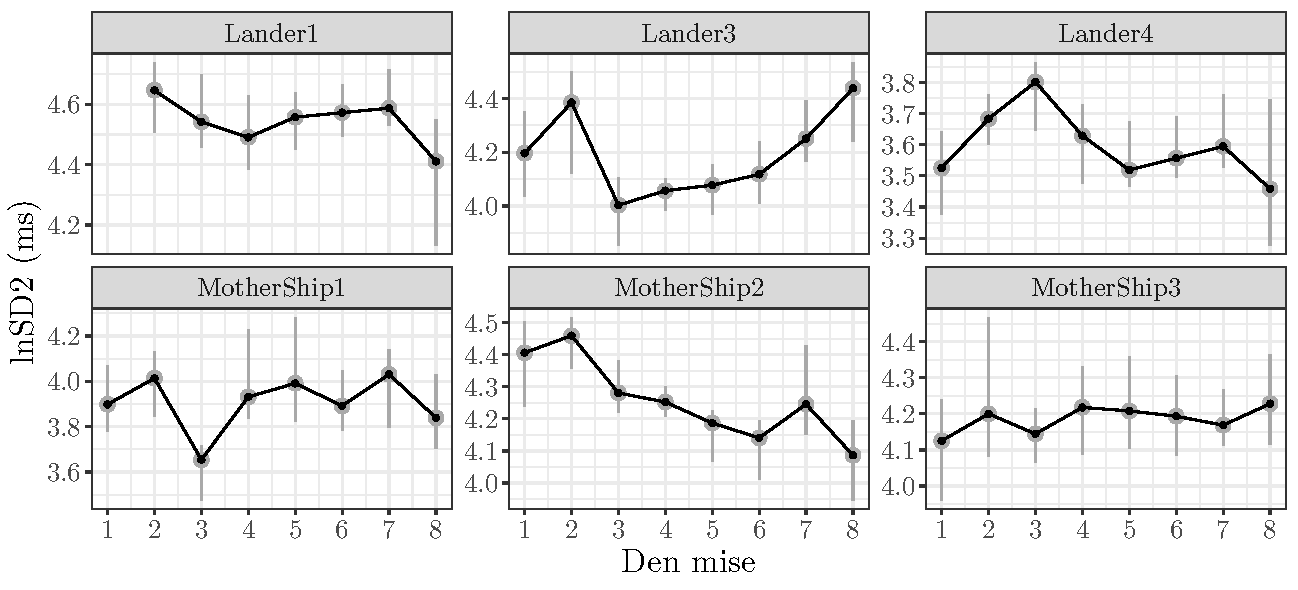
\includegraphics[width=1\linewidth]{figures/stats/pointrange_sd2.pdf}
        \caption{Medián, horní a dolní kvartil (šedý rozsah) hodnot SD2 pro jednotlivé dny}
        \label{fig:results_pointrange_sd2}
    \end{center}
    \vspace{-10mm}
\end{figure}
\begin{figure}[h]
    \begin{center}
        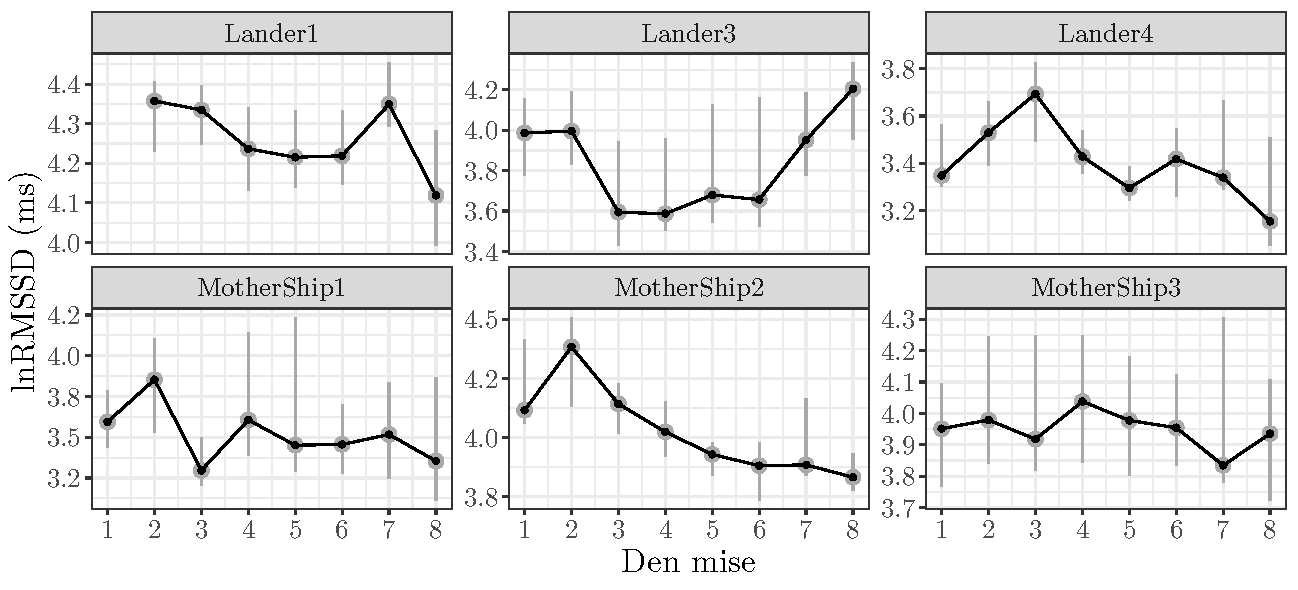
\includegraphics[width=1\linewidth]{figures/stats/pointrange_rmssd.pdf}
        \caption{Medián, horní a dolní kvartil (šedý rozsah) hodnot RMSSD pro jednotlivé dny}
        \label{fig:results_pointrange_rmssd}
    \end{center}
    \vspace{-10mm}
\end{figure}
\begin{figure}[h]
    \begin{center}
        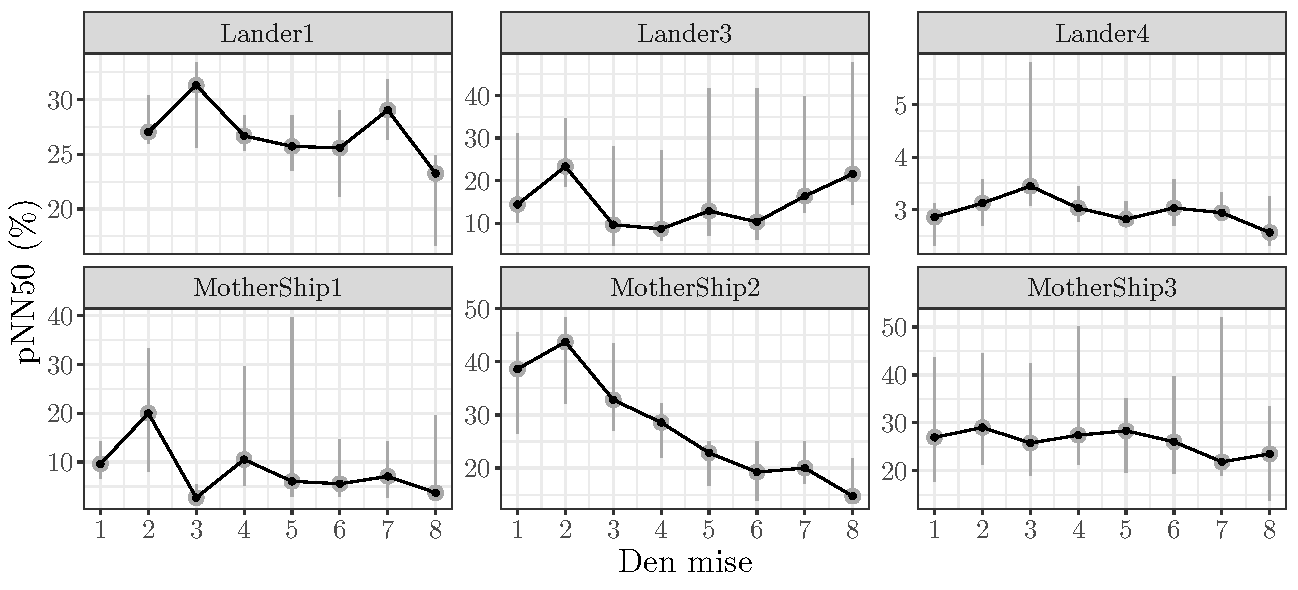
\includegraphics[width=1\linewidth]{figures/stats/pointrange_pnn50.pdf}
        \caption{Medián, horní a dolní kvartil (šedý rozsah) hodnot pNN50 pro jednotlivé dny}
        \label{fig:results_pointrange_pnn50}
    \end{center}
    \vspace{-20mm}
\end{figure}

\begin{figure}[h]
    \begin{center}
        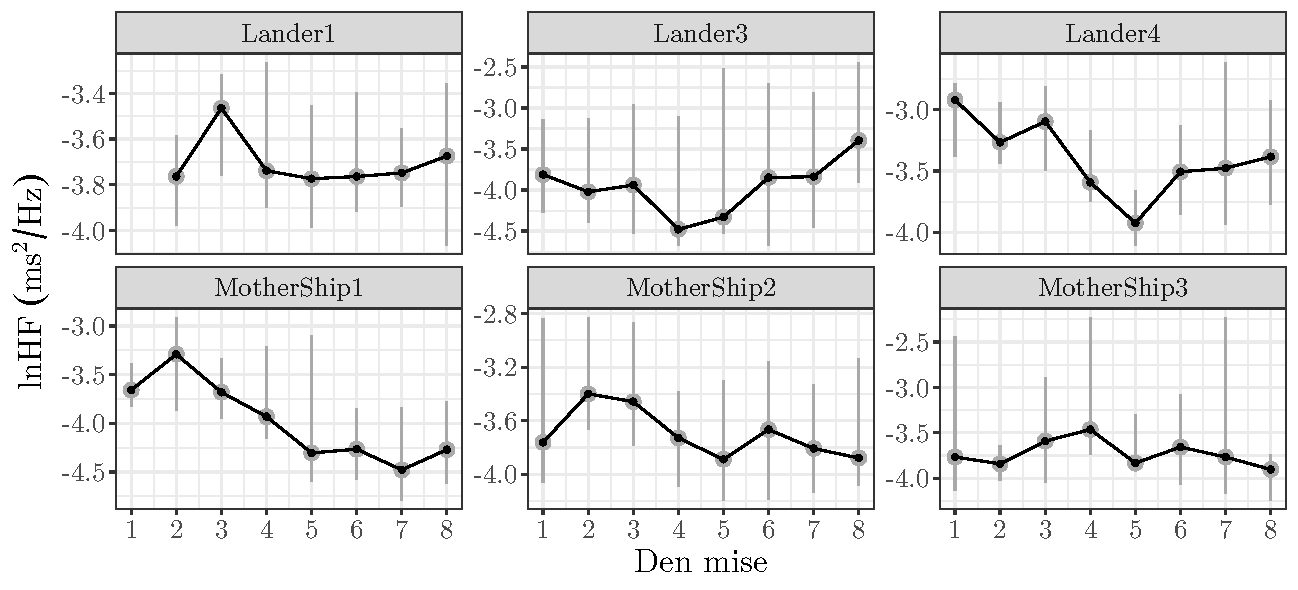
\includegraphics[width=1\linewidth]{figures/stats/pointrange_hf.pdf}
        \caption{Medián, horní a dolní kvartil (šedý rozsah) hodnot HF pro jednotlivé dny}
        \label{fig:results_pointrange_hf}
    \end{center}
\end{figure}

\subsection{Sledované veličiny během NPF stimulace}
\label{sec:result_cog_tests}
Všichni jedinci byli během mise vystaveni \gls{NPF} stimulaci ve formě baterie
kognitivních testů využitím nástroje Neurop (viz
sekce~\ref{subsubsec:neuro_testy}). Testování proběhlo dle harmonogramu mise, 
jehož příklad lze vidět na Obr.~\ref{fig:harmonogram}. Skupina přistávacího
modulu podstoupila testování třikrát v průběhu mise. Jednotlivá testování pro
tuto skupinu jsou dále v této sekci značeny následovně: F -- první testování, M
-- druhé testování a L -- třetí testování. V
Tabulce~\ref{tab:tests_params_lander} jsou uvedeny výsledky vypočtených
sledovaných veličin pro jednotlivá testování v rámci skupiny přistávacího
modulu, konkrétně průměr a směrodatná odchylka.

\begin{table}[h]
    \catcode`\-=12
    \footnotesize
    \centering
    \caption{Individuální HRV reakce analogových astronautů přistávacího modulu během neuropsychologické stimulace sadou kognitivních testů}
    \ra{1.2}
    \begin{threeparttable}
        \begin{tabular*}{\linewidth}{@{\extracolsep{\fill}} lllcccccc @{}}
            \toprule
            \textbf{Subjekt}            & \multicolumn{2}{c}{\textbf{Parametr}} & \multicolumn{2}{c}{\textbf{F}} & \multicolumn{2}{c}{\textbf{M}} & \multicolumn{2}{c}{\textbf{L}}                                                                 \\ \cmidrule(rl){4-5} \cmidrule(rl){6-7} \cmidrule(rl){8-9}
            &                                       &                                & \textbf{Průměr}                & \textbf{SD}                    & \textbf{Průměr} & \textbf{SD} & \textbf{Průměr} & \textbf{SD} \\ \midrule
            \multirow[t]{4}{*}{Lander1} & SD2                                  & (ms)                           & 83,26                          & 45,84                          & 83,48           & 43,76       & 78,22           & 40,53       \\
            & RMSSD                                 & (ms)                           & 74,14                          & 44,08                          & 80,67           & 45,11       & 71,23           & 42,12       \\
            & pNN50                                 & $(\%)$                         & 18,42                          & 14,09                          & 24,02           & 14,27       & 13,46           & 12,07       \\
            & HF                                    & ($\text{ms}^2$/Hz)             & 0,04                           & 0,03                           & 0,05            & 0,04        & 0,03            & 0,03        \\ \midrule
            \multirow[t]{4}{*}{Lander3} & SD2                                  & (ms)                           & 48,01                          & 22,92                          & 45,09           & 24,59       & 58,08           & 31,14       \\
            & RMSSD                                 & (ms)                           & 30,89                          & 13,43                          & 38,71           & 22,29       & 47,38           & 28,91        \\
            & pNN50                                 & $(\%)$                         & 5,41                           & 6,12                            & 7,07            & 6,77        & 11,74           & 8,68        \\
            & HF                                    & ($\text{ms}^2$/Hz)             & 0,03                           & 0,03                           & 0,04            & 0,03        & 0,04            & 0,04        \\ \midrule
            \multirow[t]{4}{*}{Lander4} & SD2                                  & (ms)                           & 43,97                          & 33,01                          & 44,47           & 31,31        & 32,24           & 24,33       \\
            & RMSSD                                 & (ms)                           & 41,92                          & 34,36                          & 42,74           & 31,12        & 31,17           & 25,94       \\
            & pNN50                                 & $(\%)$                         & 2,97                           & 3,83                           & 4,04            & 4,53         & 2,01            & 3,02        \\
            & HF                                    & ($\text{ms}^2$/Hz)             & 0,06                           & 0,04                           & 0,06            & 0,04        & 0,05            & 0,04        \\
            \bottomrule
        \end{tabular*}
    \end{threeparttable}
    \label{tab:tests_params_lander}
\end{table}

U jedinců ze skupiny mateřské lodi bylo testování během mise provedeno pouze
dvakrát. První testování je tedy označeno jako F a druhé jako L. Výsledky
vypočtených sledovaných veličin v rámci jednotlivých testování pro tuto skupinu
jsou uvedeny v Tabulce~\ref{tab:tests_params_mothership}.

\begin{table}[h]
    \catcode`\-=12
    \footnotesize
    \centering
    \caption{Individuální HRV reakce analogových astronautů mateřské lodi během neuropsychologické stimulace sadou kognitivních testů}
    \ra{1.2}
    \begin{threeparttable}
        \begin{tabular*}{\linewidth}{@{\extracolsep{\fill}} lllcccc @{}}
            \toprule
            \textbf{Subjekt}                & \multicolumn{2}{c}{\textbf{Parametr}} & \multicolumn{2}{c}{\textbf{F}} & \multicolumn{2}{c}{\textbf{L}}                                               \\ \cmidrule(rl){4-5} \cmidrule(rl){6-7}
            &                                       &                                & \textbf{Průměr}                & \textbf{SD} & \textbf{Průměr} & \textbf{SD} \\ \midrule
            \multirow[t]{4}{*}{MotherShip1} & SD2                                  & (ms)                           & 31,63                          & 14,12          & 51,07           & 25,17       \\
            & RMSSD                                 & (ms)                           & 22,99                          & 11,9        & 41,28           & 26,39       \\
            & pNN50                                 & $(\%)$                         & 2,56                           & 3,89        & 5,68            & 6,97        \\
            & HF                                    & ($\text{ms}^2$/Hz)                    & 0,04                           & 0,04        & 0,02            & 0,02        \\ \midrule
            \multirow[t]{4}{*}{MotherShip2} & SD2                                  & (ms)                           & 94,54                          & 38,23       & 72,81           & 36,67       \\
            & RMSSD                                 & (ms)                           & 76,61                           & 33,23       & 56,12            & 31,51       \\
            & pNN50                                 & $(\%)$                         & 33,55                          & 11,62       & 22,64           & 13,66       \\
            & HF                                    & ($\text{ms}^2$/Hz)                    & 0,03                           & 0,03        & 0,03            & 0,03        \\ \midrule
            \multirow[t]{4}{*}{MotherShip3} & SD2                                  & (ms)                           & 64,67                          & 22,84       & 64,52           & 27,04       \\
            & RMSSD                                 & (ms)                           & 50,88                          & 15,73       & 46,57           & 22,13       \\
            & pNN50                                 & $(\%)$                         & 23,68                          & 6,88        & 17,55           & 8,92        \\
            & HF                                    & ($\text{ms}^2$/Hz)                    & 0,03                           & 0,02        & 0,02            & 0,02        \\
            \bottomrule
        \end{tabular*}
    \end{threeparttable}
    \label{tab:tests_params_mothership}
\end{table}

Jak již bylo popsáno v sekci~\ref{sec:zpracovani_dat_diana}, každé sezení, během
kterého jedinec podstoupil \gls{NPF} stimulaci sadou kognitivních testů, bylo na
úrovni zaznamenaných biosignálu během testování segmentováno a zpracováno. Ve
zbytku této sekce jsou vizualizovány zpracovaná data jednotlivých testování pro
každého jedince ve formě krabicových grafů pro všechny sledované veličiny.

\begin{figure}[h]
    \begin{center}
        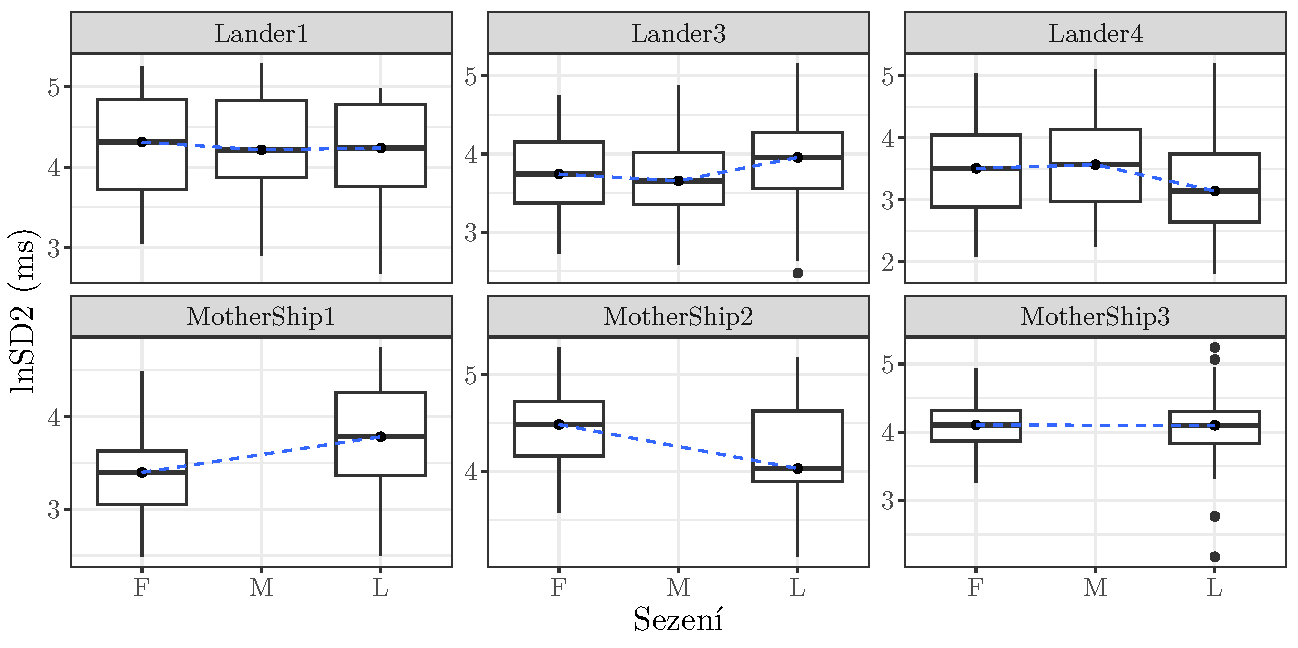
\includegraphics[width=1\linewidth]{figures/stats/boxplot_sd2_tests.pdf}
        \caption{Krabicové grafy pro parametr SD2 během jednotlivých NPF testování}
        \label{fig:results_boxplot_SD2_tests}
    \end{center}
    \vspace{-20mm}
\end{figure}

\begin{figure}[H]
    \begin{center}
        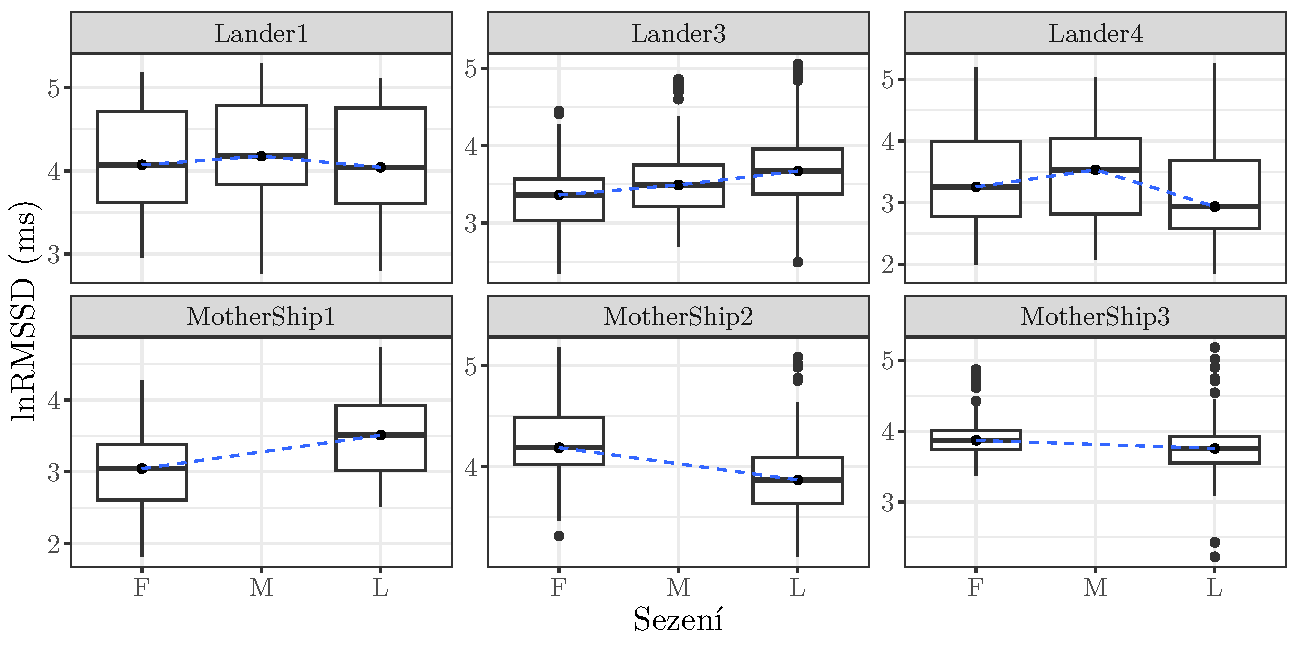
\includegraphics[width=1\linewidth]{figures/stats/boxplot_rmssd_tests.pdf}
        \caption{Krabicové grafy pro parametr RMSSD během jednotlivých NPF testování}
        \label{fig:results_boxplot_rmssd_tests}
    \end{center}
    \vspace{-12mm}
\end{figure}
\begin{figure}[H]
    \begin{center}
        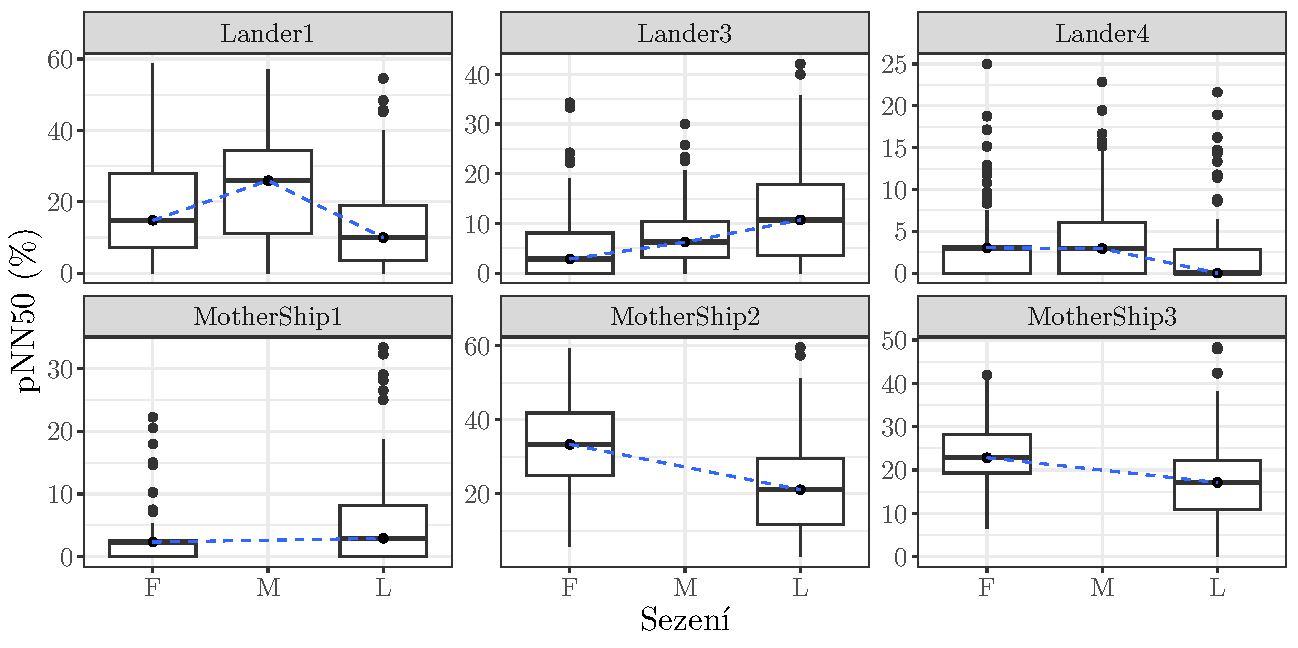
\includegraphics[width=1\linewidth]{figures/stats/boxplot_pnn50_tests.pdf}
        \caption{Krabicové grafy pro parametr pNN50 během jednotlivých NPF testování}
        \label{fig:results_boxplot_pnn50_tests}
    \end{center}
    \vspace{-12mm}
\end{figure}
\begin{figure}[H]
    \begin{center}
        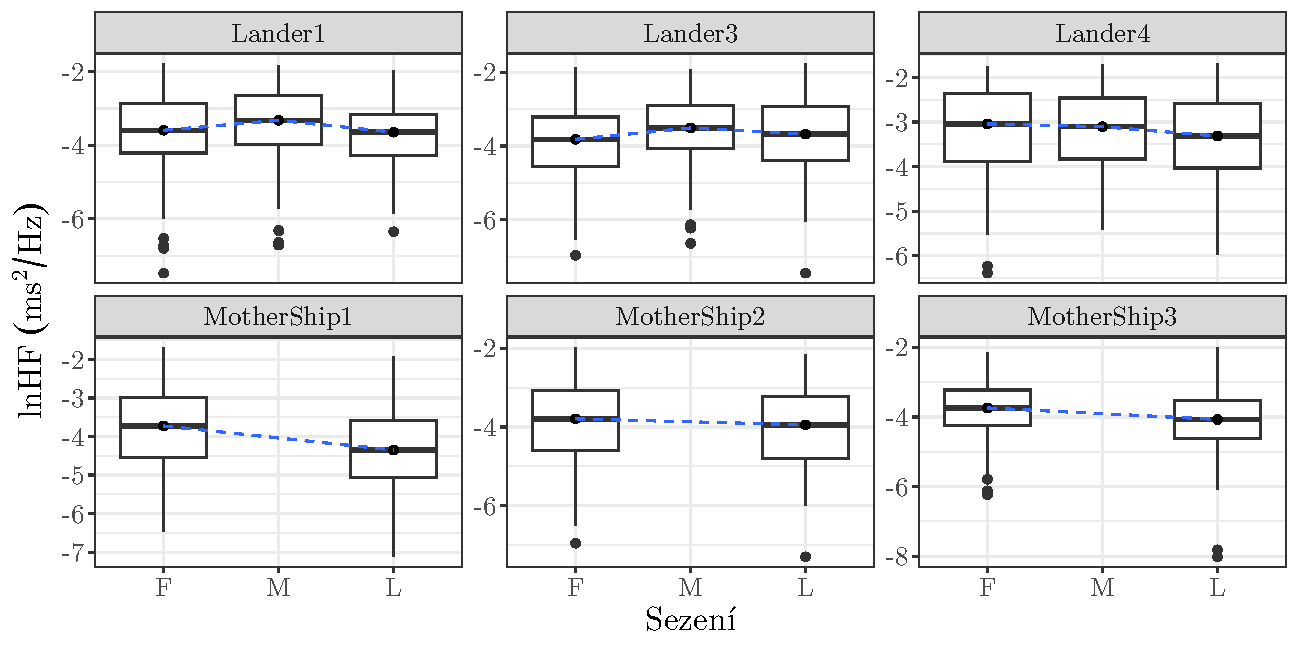
\includegraphics[width=1\linewidth]{figures/stats/boxplot_hf_tests.pdf}
        \caption{Krabicové grafy pro parametr HF během jednotlivých NPF testování}
        \label{fig:results_boxplot_hf_tests}
    \end{center}
    \vspace{-20mm}
\end{figure}

\subsection{Statistické modelování}
\label{sec:vysledky_lmm}
V této sekci jsou uvedeny výsledky statistického modelování sledovaných veličin
využitím lineárních smíšených modelů (viz sekce~\ref{subsec:tvorba_modelů}
a~\ref{subsec:lmm}). V Tabulce~\ref{tab:lmm_rmssd_SD2} jsou uvedeny výsledky
\gls{LMM} pro parametry SD2 a RMSSD. V tabulkách označuje proměnná
$\mathrm{N}_{\text{id}}$ počet pozorovaných subjektů.

\begin{table}[h]
    \catcode`\-=12
    \footnotesize
    \centering
    \caption{Fixní efekty lineárních smíšených modelů pro parametry SD2 a RMSSD}
    \ra{1.2}
    \begin{threeparttable}
        \begin{tabular*}{\linewidth}{@{\extracolsep{\fill}} lcccccc @{}}
            \toprule
            & \multicolumn{3}{c}{\textbf{lnSD2}} & \multicolumn{3}{c}{\textbf{lnRMSSD}}                                                                      \\ \cmidrule(rl){2-4} \cmidrule(rl){5-7}
            \textit{Prediktor}          & \textit{Odhad}                      & \textit{95\%~CI}                          & \textit{p}      & \textit{Odhad} & \textit{95\%~CI}   & \textit{p}      \\ \midrule
            (Intercept)                 & 4,18                                & 2,88 -- 5,48                         & \textbf{<0,001} & 4,01           & 3,70 -- 4,33  & \textbf{<0,001} \\
            Den                         & -0,01                               & -0,03 -- 0,01                        & 0,318           & -0,03          & -0,05 -- 0,00 & \textbf{0,023}  \\
            Skupina Lander              & -0,08                               & -0,56 -- 0,40                        & 0,742           & -0,11          & -0,55 -- 0,35 & 0,654           \\
            Den $\times$ skupina Lander & 0,01                                & -0,02 -- 0,04                        & 0,424           & 0,02           & -0,01 -- 0,05 & 0,244           \\ \midrule
            $\mathrm{N}_{\text{id}}$    & \multicolumn{3}{c}{6}               & \multicolumn{3}{c}{6}                                                                                     \\
            Počet pozorování            & \multicolumn{3}{c}{3870}            & \multicolumn{3}{c}{3866}                                                                                  \\
            \bottomrule
        \end{tabular*}
    \end{threeparttable}
    \label{tab:lmm_rmssd_SD2}
\end{table}

\begin{figure}[!htb]
    \centering
    \begin{subfigure}[h]{0.43\linewidth}
        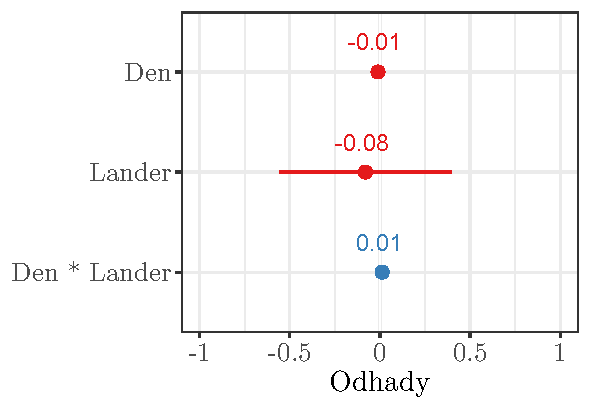
\includegraphics[width=\linewidth]{figures/stats/lmm_sd2_coef}
        \caption{Pro parametr SD2}
    \end{subfigure}
    \hfill
    \begin{subfigure}[h]{0.43\linewidth}
        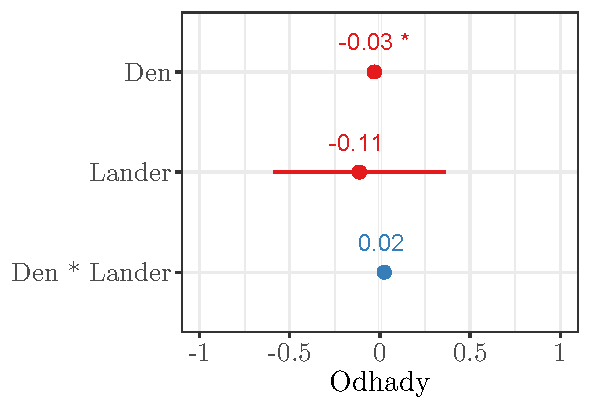
\includegraphics[width=\linewidth]{figures/stats/lmm_rmssd_coef}
        \caption{Pro parametr RMSSD}
    \end{subfigure}
    \caption{Vizualizace odhadů (fixních efektů) navržených modelů}
    \label{fig:results_lmm_coefs1}
\end{figure}

\begin{figure}[!htb]
    \begin{center}
        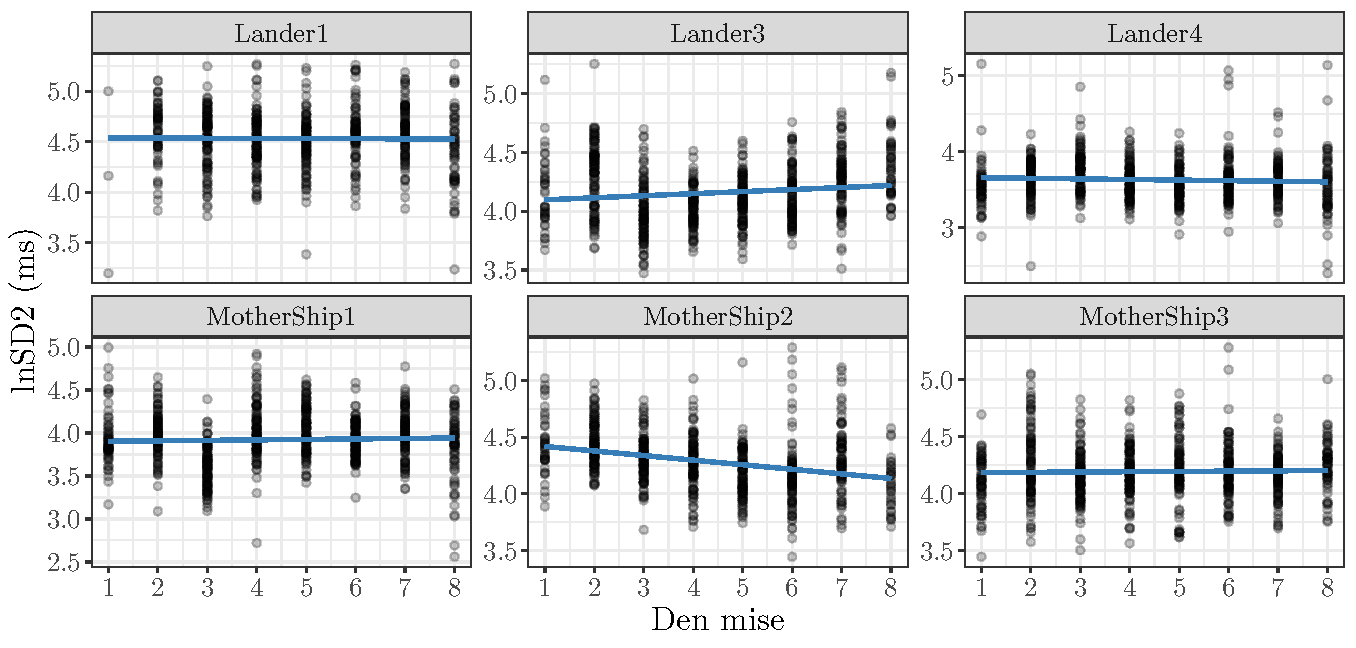
\includegraphics[width=1\linewidth]{figures/stats/lmm_sd2_fit}
        \caption{Grafická reprezentace modelu pro parametr SD2 na individuální úrovni}
        \label{fig:results_lmm_fit1}
    \end{center}
    \vspace{-10mm}
\end{figure}

\begin{figure}[!htb]
    \begin{center}
        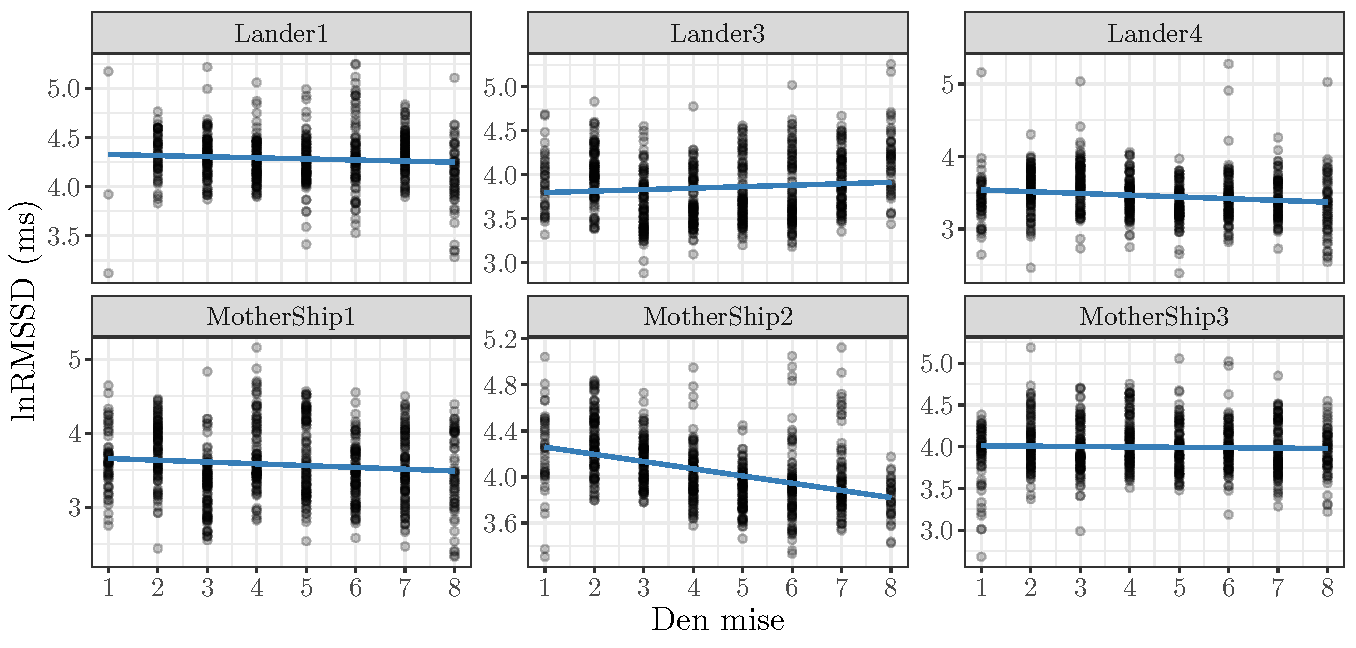
\includegraphics[width=1\linewidth]{figures/stats/lmm_rmssd_fit}
        \caption{Grafická reprezentace modelu pro parametr RMSSD na individuální úrovni}
        \label{fig:results_lmm_fit2}
    \end{center}
\end{figure}

V Tabulce~\ref{tab:lmm_pnn50_hf} jsou uvedeny výsledky modelování pro parametry
pNN50 a HF. V tabulkách opět označuje proměnná $\mathrm{N}_{\text{id}}$ počet
pozorovaných subjektů. Byly vytvořeny i grafické reprezentace fixních efektů pro
každý model zvlášť včetně příkladů grafů modelů lineárních smíšených efektů v
rámci každého subjektu. Všechny grafy jsou uvedeny v návaznosti na patřičnou
tabulku výsledků \gls{LMM}.

\begin{table}[h]
    \catcode`\-=12
    \footnotesize
    \centering
    \caption{Fixní efekty lineárních smíšených modelů pro parametry pNN50 a HF}
    \ra{1.2}
    \begin{threeparttable}
        \begin{tabular*}{\linewidth}{@{\extracolsep{\fill}} lcccccc @{}}
            \toprule
            & \multicolumn{3}{c}{\textbf{pNN50}} & \multicolumn{3}{c}{\textbf{lnHF}}                                                                       \\ \cmidrule(rl){2-4} \cmidrule(rl){5-7}
            \textit{Prediktor}          & \textit{Odhad}                     & \textit{95\%~CI}                       & \textit{p}      & \textit{Odhad} & \textit{95\%~CI}    & \textit{p}      \\ \midrule
            (Intercept)                 & 30,69                              & 18,50 -- 43,88                    & \textbf{<0,001} & -3,32          & -3,57 -- -3,07 & \textbf{<0,001} \\
            Den                         & -1,44                              & -2,70 -- -0,19                    & \textbf{0,024}           & -0,07          & -0,12 -- -0,02 & \textbf{0,004}  \\
            Skupina Lander              & -13,05                             & -30,30 -- 4,20                    & 0,138           & -0,24          & -0,59 -- 0,11  & 0,179           \\
            Den $\times$ skupina Lander & 1,41                               & -0,38 -- 3,19                     & 0,122           & 0,06           & 0,01 -- 0,13   & 0,083           \\ \midrule
            $\mathrm{N}_{\text{id}}$    & \multicolumn{3}{c}{6}              & \multicolumn{3}{c}{6}                                                                                   \\
            Počet pozorování            & \multicolumn{3}{c}{3874}           & \multicolumn{3}{c}{3974}                                                                                \\
            \bottomrule
        \end{tabular*}
    \end{threeparttable}
    \label{tab:lmm_pnn50_hf}
\end{table}

\begin{figure}[!htb]
    \centering
    \begin{subfigure}[h]{0.43\linewidth}
        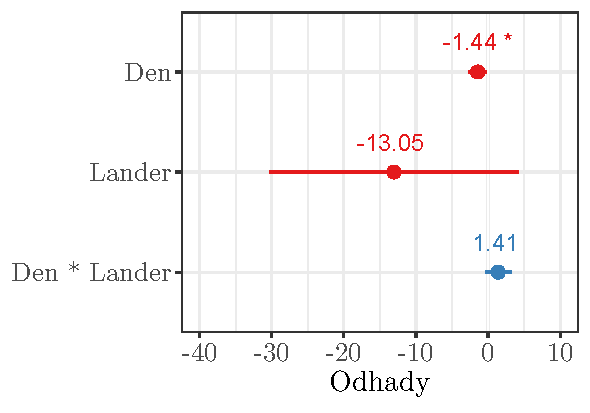
\includegraphics[width=\linewidth]{figures/stats/lmm_pnn50_coef}
        \caption{Pro parametr pNN50}
    \end{subfigure}
    \hfill
    \begin{subfigure}[h]{0.43\linewidth}
        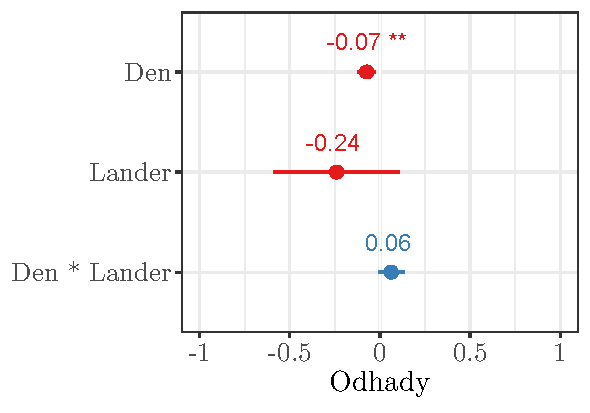
\includegraphics[width=\linewidth]{figures/stats/lmm_hf_coef}
        \caption{Pro parametr HF}
    \end{subfigure}
    \caption{Vizualizace odhadů (fixních efektů) navržených modelů}
    \label{fig:results_lmm_coefs2}
\end{figure}

\begin{figure}[!htb]
    \begin{center}
        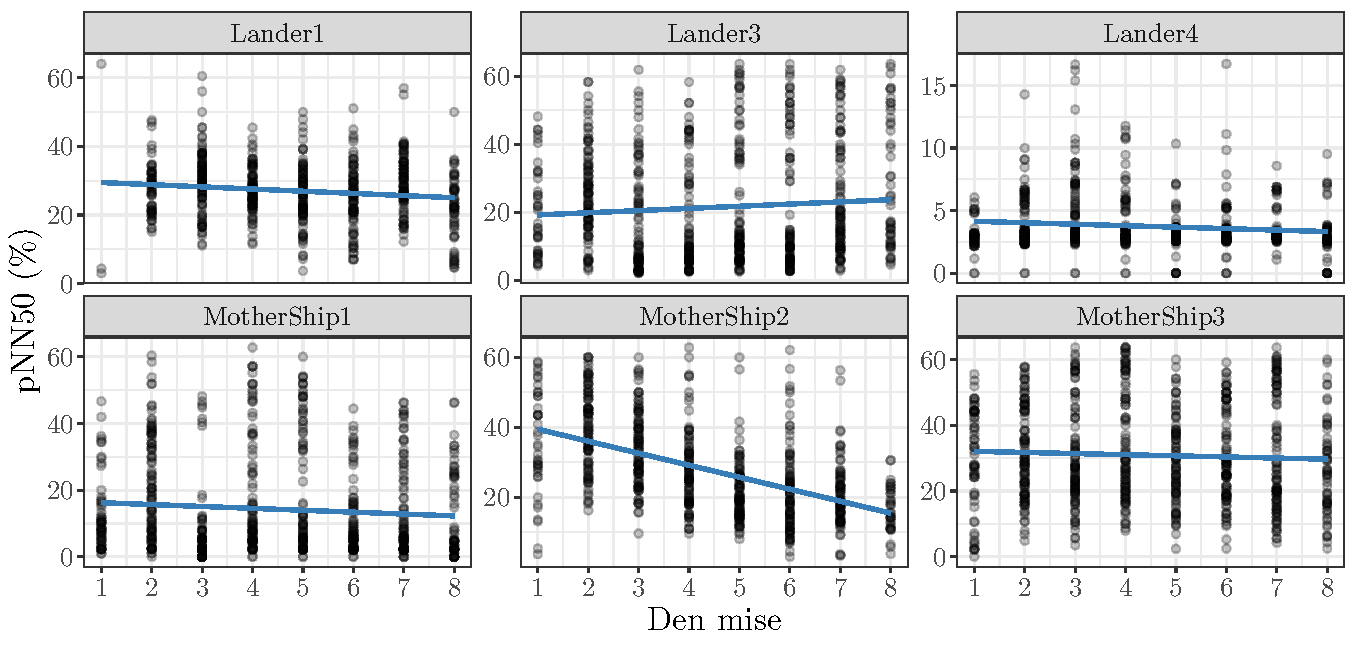
\includegraphics[width=1\linewidth]{figures/stats/lmm_pnn50_fit}
        \caption{Grafická reprezentace modelu pro parametr pNN50 na individuální úrovni}
        \label{fig:results_lmm_fit3}
    \end{center}
\end{figure}

\begin{figure}[!htb]
    \begin{center}
        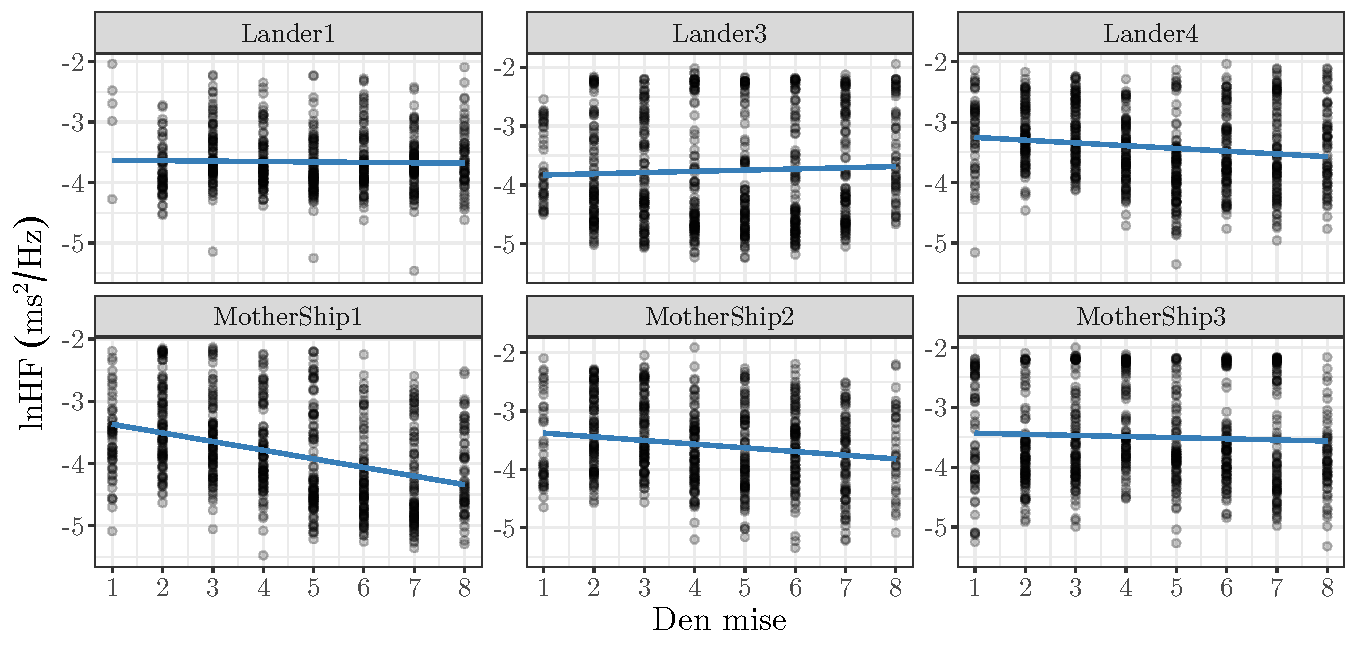
\includegraphics[width=1\linewidth]{figures/stats/lmm_hf_fit}
        \caption{Grafická reprezentace modelu pro parametr HF na individuální úrovni}
        \label{fig:results_lmm_fit4}
    \end{center}
\end{figure}



\section{Modely pro hodnocení kognitivní zátěže}
\label{sec:vysledky_detekce_cl}
V této sekci jsou prezentovány výsledky části strojového učení. Nejprve jsou
uvedeny výsledky trénování modelů využitím navržené metody pro hodnocení
kognitivní zátěže (viz sekce~\ref{sec:hybridni_detekce}). Výsledky jsou uvedeny
zvláště pro každý benchmarkovací dataset a poté pro sjednocené datasety. Popis
jednotlivých datasetů se nachází v sekci~\ref{sec:datasety}.

Poslední dvě části sekce jsou věnovány porovnání navrženého řešení se současným
stavem a experimentálnímu ověření řešení. Ověření je realizováno na datech z
analogové vesmírné mise DIANA, konkrétně na úsecích, kdy byl subjekt podroben
\gls{NPF} stimulaci. Všechny experimenty jsou součásti přílohy diplomové práce.

\subsection{Hodnocení přesnosti modelů pro WESAD}
\label{subsec:wesad_models}
V této sekci jsou uvedeny výsledky z trénování modelů na datasetu WESAD v podobě
vybraných hodnotících metrik (viz sekce~\ref{subsec:ml_metriky}), matic záměn a
ROC křivek. Matice záměn byly normalizovány na relativní četnosti v rámci
sloupců. Matice pro augmentované (Aug.) verze datasetů jsou uvedeny v
Příloze~\ref{appendix:b}.

\begin{table}[h]
    \small
    \centering
    \caption{Výsledky hodnocení přesnosti modelů WESAD (Acc. = přesnost)}
    \ra{1.2}
    \begin{tabular*}{\linewidth}{@{\extracolsep{\fill}} r| c | lllll @{}}
        \toprule
        Model                       & Aug. & Acc.     & Test acc. & TPR      & TNR      & AUC   \\ \midrule
        \multirow{2}{*}{WESAD-5s}   & Ne   & 99,75~\% & 95,46~\%  & 95,21~\% & 90,07~\% & 0,926 \\
        & Ano  & 99,91~\% & 97,73~\%  & 97,51~\% & 97,54~\% & 0,986 \\ \midrule
        \multirow{2}{*}{WESAD-5s50} & Ne   & 99.93~\% & 96,84~\%  & 95,63~\% & 94,57~\% & 0,986 \\
        & Ano  & 99,97~\% & 98,25~\%  & 98,06~\% & 98,06~\% & 0,996 \\ \midrule
        \multirow{2}{*}{WESAD-1s}   & Ne   & 99,45~\% & 95,25~\%  & 91,60~\% & 93,81~\% & 0,981 \\
        & Ano  & 99,73~\% & 96,66~\%  & 95,61~\% & 95,23~\% & 0,996 \\
        \bottomrule
    \end{tabular*}
    \label{tab:wesad_eval}
\end{table}

\begin{figure}[!htb]
    \centering
    \begin{subfigure}[h]{0.32\linewidth}
        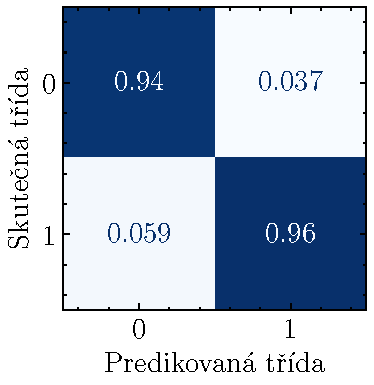
\includegraphics[width=\linewidth]{figures/wesad/wesad_5s}
        \caption{WESAD-5s}
    \end{subfigure}
    \hspace{0.05cm}
    \begin{subfigure}[h]{0.32\linewidth}
        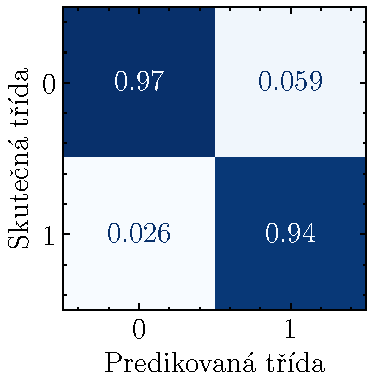
\includegraphics[width=\linewidth]{figures/wesad/wesad_5s50}
        \caption{WESAD-5s50}
    \end{subfigure}
    \hspace{0.05cm}
    \begin{subfigure}[h]{0.32\linewidth}
        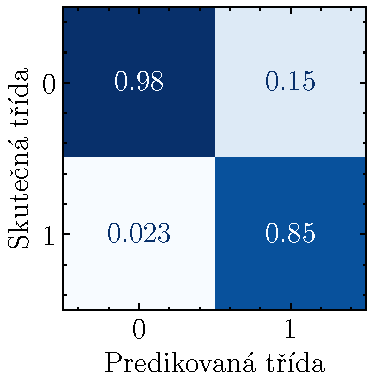
\includegraphics[width=\linewidth]{figures/wesad/wesad_1s}
        \caption{WESAD-1s}
    \end{subfigure}
    \caption{Matice záměn pro WESAD modely (0 = klidový stav, 1 = CL stav)}
    \label{fig:results_cm_wesad}
\end{figure}

\begin{figure}[!htb]
    \centering
    \begin{subfigure}[h]{0.42\linewidth}
        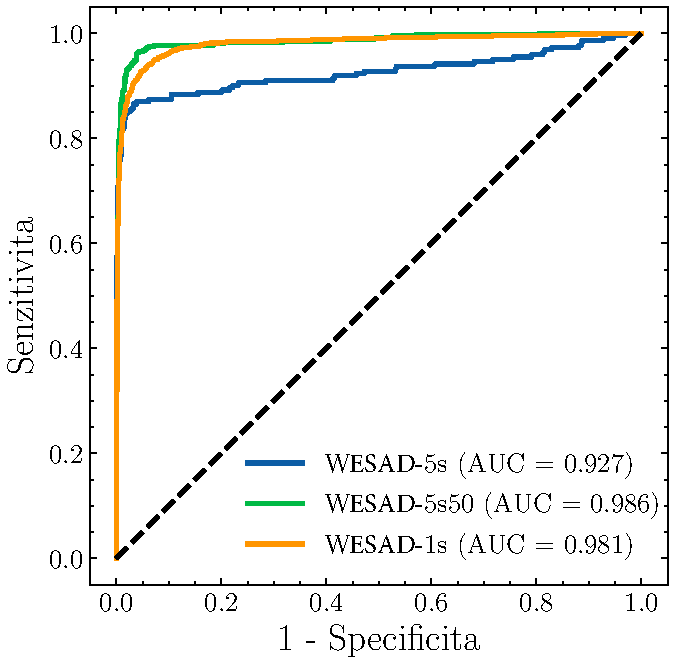
\includegraphics[width=\linewidth]{figures/wesad/wesad_roc}
        \caption{WESAD}
    \end{subfigure}
    \hspace{0.1cm}
    \begin{subfigure}[h]{0.42\linewidth}
        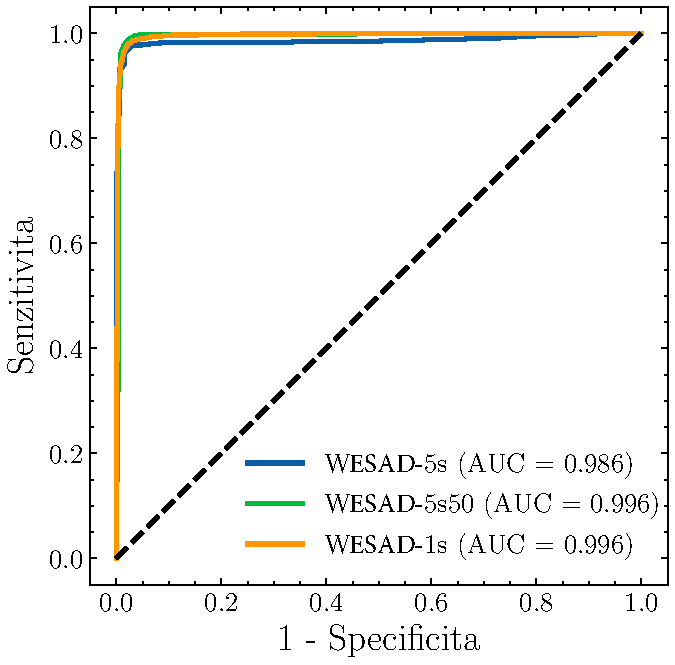
\includegraphics[width=\linewidth]{figures/wesad/wesad_roc_aug}
        \caption{WESAD s augmentací}
    \end{subfigure}
    \caption{ROC křivky pro WESAD modely}
    \label{fig:results_roc_wesad}
\end{figure}


\subsection{Hodnocení přesnosti modelů pro CLAS}
\label{subsec:clas_models}
V této sekci jsou uvedeny výsledky z trénování modelů na datasetu CLAS v podobě
vybraných hodnotících metrik (viz sekce~\ref{subsec:ml_metriky}), matic záměn a
ROC křivek. Matice záměn byly normalizovány na relativní četnosti v rámci
sloupců. Matice pro augmentované (Aug.) verze datasetů jsou uvedeny v
Příloze~\ref{appendix:b}.

\begin{table}[h]
    \small
    \centering
    \caption{Výsledky hodnocení přesnosti modelů CLAS (Acc. = přesnost)}
    \ra{1.2}
    \begin{tabular*}{\linewidth}{@{\extracolsep{\fill}} r|c|lllll @{}}
        \toprule
        Model                      & Aug. & Acc.     & Test acc. & TPR      & TNR      & AUC   \\ \midrule
        \multirow{2}{*}{CLAS-5s}   & Ne   & 99,35~\% & 91,79~\%  & 77,67~\% & 54,14~\% & 0,994 \\
        & Ano  & 99,91~\% & 97,45~\%  & 97,21~\% & 97,17~\% & 0,994 \\ \midrule
        \multirow{2}{*}{CLAS-5s50} & Ne   & 99,43~\% & 92,17~\%  & 75,99~\% & 57,68~\% & 0,756 \\
        & Ano  & 99,89~\% & 97,87~\%  & 97,66~\% & 97,65~\% & 0,996 \\ \midrule
        \multirow{2}{*}{CLAS-1s}   & Ne   & 97,91~\% & 92,04~\%  & 81,29~\% & 53,67~\% & 0,667 \\
        & Ano  & 98,21~\% & 96,55~\%  & 96,46~\% & 96,46~\% & 0,992 \\
        \bottomrule
    \end{tabular*}
    \label{tab:clas_eval}
\end{table}

\begin{figure}[!htb]
    \centering
    \begin{subfigure}[h]{0.32\linewidth}
        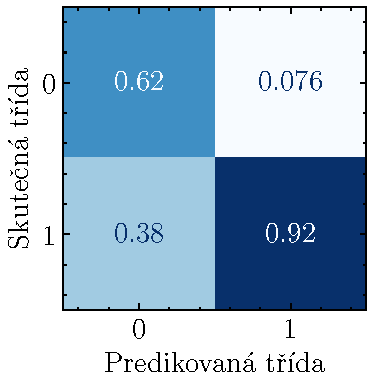
\includegraphics[width=\linewidth]{figures/clas/clas_5s}
        \caption{CLAS-5s}
    \end{subfigure}
    \hspace{0.05cm}
    \begin{subfigure}[h]{0.32\linewidth}
        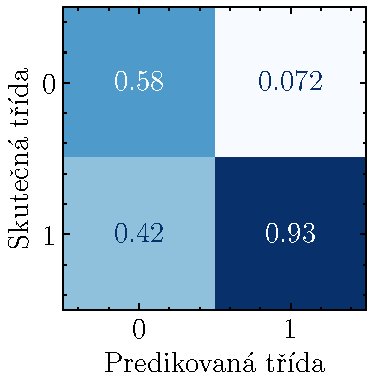
\includegraphics[width=\linewidth]{figures/clas/clas_5s50}
        \caption{CLAS-5s50}
    \end{subfigure}
    \hspace{0.05cm}
    \begin{subfigure}[h]{0.32\linewidth}
        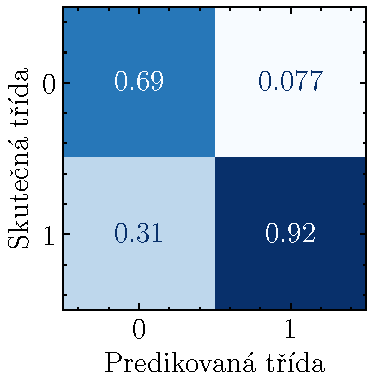
\includegraphics[width=\linewidth]{figures/clas/clas_1s}
        \caption{CLAS-1s}
    \end{subfigure}
    \caption{Matice záměn pro CLAS modely (0 = klidový stav, 1 = CL stav)}
    \label{fig:results_cm_clas}
\end{figure}

\begin{figure}[!htb]
    \centering
    \begin{subfigure}[h]{0.42\linewidth}
        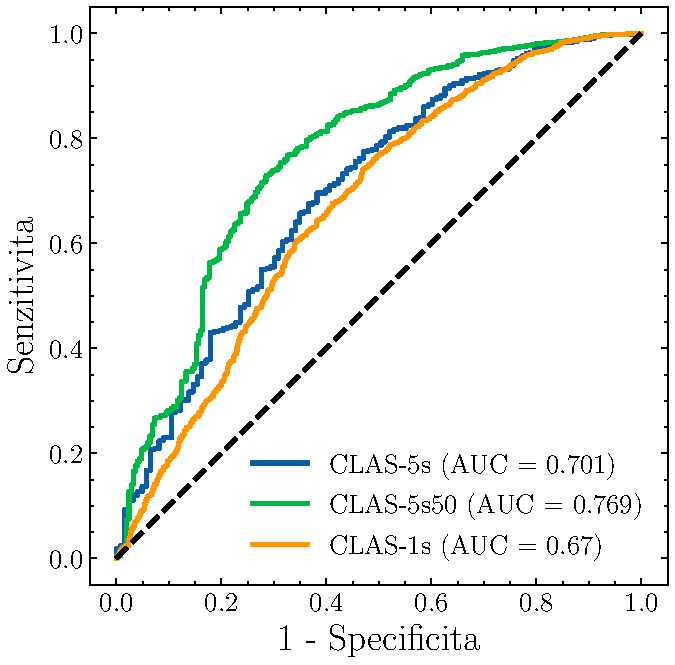
\includegraphics[width=\linewidth]{figures/clas/clas_roc}
        \caption{CLAS}
    \end{subfigure}
    \hspace{0.1cm}
    \begin{subfigure}[h]{0.42\linewidth}
        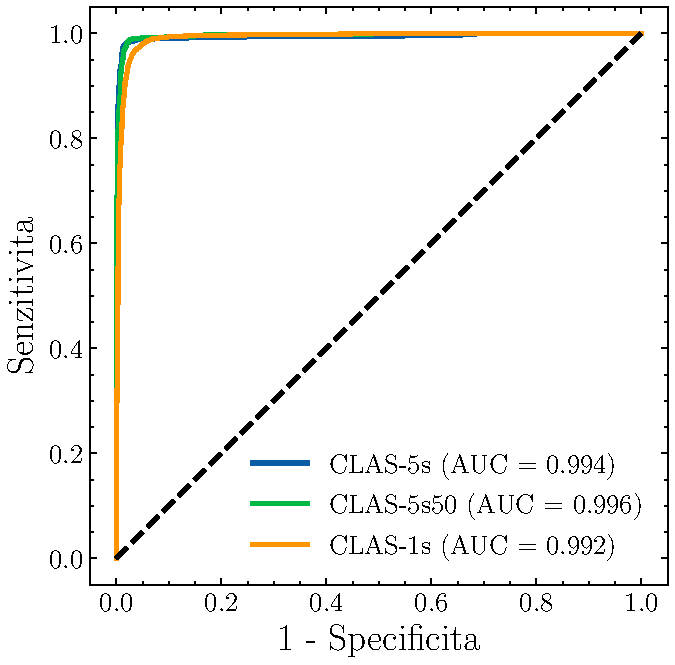
\includegraphics[width=\linewidth]{figures/clas/clas_roc_aug}
        \caption{CLAS s augmentací}
    \end{subfigure}
    \caption{ROC křivky pro CLAS modely}
    \label{fig:results_roc_clas}
\end{figure}

\subsection{Hodnocení přesnosti modelů pro sjednocená data}
\label{subsec:merged_models}
V této sekci jsou uvedeny výsledky z trénování modelů na sloučených datasetech
(dále jen Merged) v podobě vybraných hodnotících metrik (viz
sekce~\ref{subsec:ml_metriky}), matic záměn a ROC křivek. Matice záměn byly
normalizovány na relativní četnosti v rámci sloupců. Matice pro augmentované
(Aug.) verze datasetů jsou v příloze~\ref{appendix:b}.

\begin{table}[h]
    \small
    \centering
    \caption{Výsledky hodnocení přesnosti modelů Merged (Acc. = přesnost)}
    \ra{1.2}
    \begin{tabular*}{\linewidth}{@{\extracolsep{\fill}} r|c|lllll @{}}
        \toprule
        Model                        & Aug. & Acc.     & Test acc. & TPR      & TNR      & AUC   \\ \midrule
        \multirow{2}{*}{Merged-5s}   & Ne   & 98,65~\% & 91,96~\%  & 92,16~\% & 88,63~\% & 0,937 \\
        & Ano  & 99,74~\% & 96,16~\%  & 95,89~\% & 95,90~\% & 0,989 \\ \midrule
        \multirow{2}{*}{Merged-5s50} & Ne   & 98,81~\% & 92,96~\%  & 92,91~\% & 90,70~\% & 0,944 \\
        & Ano  & 99,73~\% & 97,55~\%  & 96,99~\% & 96,88~\% & 0,991 \\ \midrule
        \multirow{2}{*}{Merged-1s}   & Ne   & 96,65~\% & 93,61~\%  & 93,77~\% & 91,99~\% & 0,952 \\
        & Ano  & 99,16~\% & 97,24~\%  & 97,13~\% & 97,12~\% & 0,992 \\
        \bottomrule
    \end{tabular*}
    \label{tab:merged}
\end{table}

\begin{figure}[!htb]
    \centering
    \begin{subfigure}[h]{0.32\linewidth}
        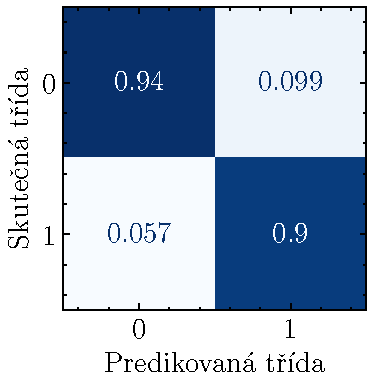
\includegraphics[width=\linewidth]{figures/merged/merged_5s}
        \caption{Merged-5s}
    \end{subfigure}
    \hspace{0.05cm}
    \begin{subfigure}[h]{0.32\linewidth}
        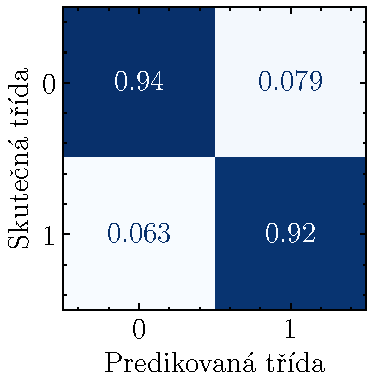
\includegraphics[width=\linewidth]{figures/merged/merged_5s50}
        \caption{Merged-5s50}
    \end{subfigure}
    \hspace{0.05cm}
    \begin{subfigure}[h]{0.32\linewidth}
        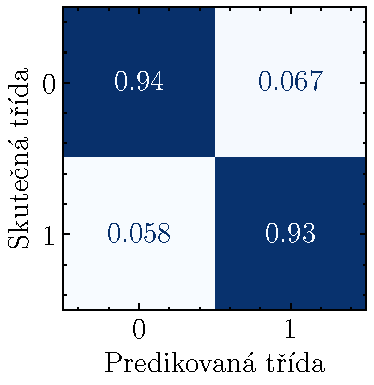
\includegraphics[width=\linewidth]{figures/merged/merged_1s}
        \caption{Merged-1s}
    \end{subfigure}
    \caption{Matice záměn pro Merged modely (0 = klidový stav, 1 = CL stav)}
    \label{fig:results_cm_merged}
\end{figure}

\begin{figure}[!htb]
    \centering
    \begin{subfigure}[h]{0.42\linewidth}
        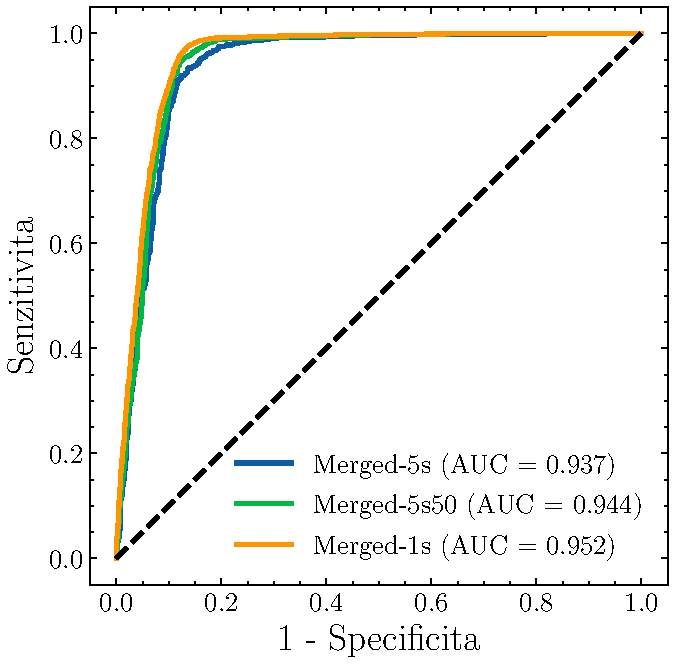
\includegraphics[width=\linewidth]{figures/merged/merged_roc}
        \caption{Merged}
    \end{subfigure}
    \hspace{0.1cm}
    \begin{subfigure}[h]{0.42\linewidth}
        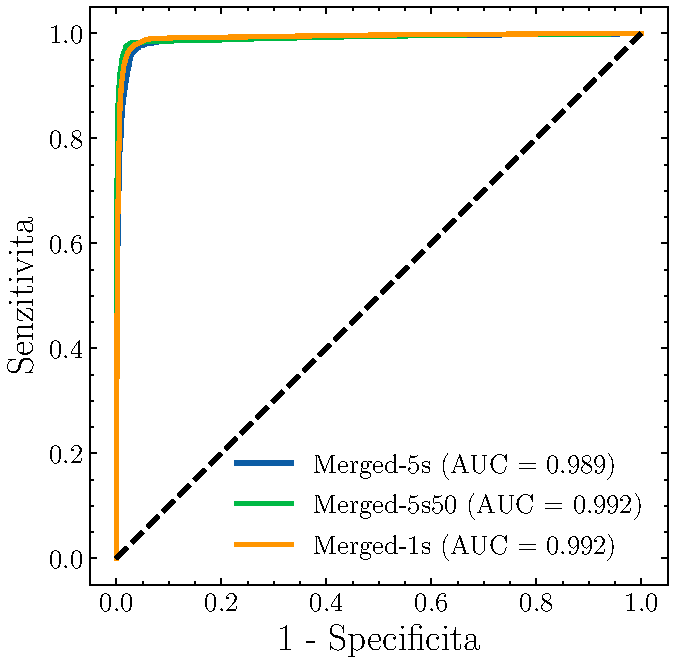
\includegraphics[width=\linewidth]{figures/merged/merged_roc_aug}
        \caption{Merged s augmentací}
    \end{subfigure}
    \caption{ROC křivky pro Merged modely}
    \label{fig:results_roc_merged}
\end{figure}

\subsection{Srovnání na úrovni použitých modalit}
\label{subsec:features_comparison}
V následující tabulce jsou uvedeny výsledky z trénování na sloučených datasetech
(Merged-5s) s různými kombinacemi modalit pro účely porovnání jejich
významnosti.

\begin{table}[h]
    \small
    \centering
    \caption{Výsledky hodnocení důležitosti využitých modalit pro hodnocení
        kognitivní zátěže v rámci modelu Merged-5s (Acc. = přesnost)}
    \ra{1.2}
    \begin{tabular*}{\linewidth}{@{\extracolsep{\fill}} llllll @{}}
        \toprule
        Modality            & Acc.     & Test acc. & TPR      & TNR      & AUC   \\ \midrule
        EKG, RSP, EDA       & 98,65~\% & 91,96~\%  & 92,16~\% & 88,63~\% & 0,937 \\
        EKG, RSP            & 96,17~\% & 90,52~\%  & 84,88~\% & 74,52~\% & 0,865 \\
        EKG, EDA            & 97,41~\% & 91,75~\%  & 87,91~\% & 79,89~\% & 0,895 \\
        EKG                 & 95,99~\% & 89,57~\%  & 77,31~\% & 76,05~\% & 0,766 \\
        RSP                 & 91,47~\% & 87,96~\%  & 50,12~\% & 50,06~\% & 0,511 \\
        EDA                 & 92,23~\% & 89,07~\%  & 42,68~\% & 45,46~\% & 0,519 \\
        \bottomrule
    \end{tabular*}
    \label{tab:features}
\end{table}

\subsection{Srovnání se současným stavem}
\label{subsec:state_comparison}
Navržené řešení v této práci bylo porovnáno s vybranými dosavadními přístupy,
jež využívají strojového učení pro rozpoznání kognitivní zátěže. Srovnání lze
vidět v Tab.~\ref{tab:state_comparison}. Všechna řešení využívají minimálně
jednu modalitu (primárně EKG).

\begin{table}[h]
    \small
    \centering
    \caption{Výsledky srovnání s dosavadními přístupy}
    \ra{1.2}
    \begin{threeparttable}
        \begin{tabular*}{\linewidth}{@{\extracolsep{\fill}} lcccc @{}}
            \toprule
            Autor                                   & Dataset & Okno & Test acc. & Rok  \\ \midrule
            Feradov et al.~\cite{Feradov2020}       & CLAS    & 30s  & 84~\%     & 2020 \\
            Ahmad et al.~\cite{Ahmad2021}           & WESAD   & 1s   & 72~\%     & 2021 \\
            Garg et al.~\cite{Garg2021}             & WESAD   & 10s  & 84~\%     & 2021 \\
            Rabbani et al.~\cite{Rabbani2022}       & WESAD   & 10s  & 87~\%     & 2022 \\
            Zhu et al.~\cite{Zhu2022}               & CLAS    & 30s  & 86~\%     & 2022 \\
            *Quadrini et al.~\cite{Quadrini2022}    & WESAD   & 60s  & 91~\%     & 2022 \\
            Chatterjee et al.~\cite{Chatterjee2022} & WESAD   & 30s  & 94~\%     & 2022 \\
            Dair et al.~\cite{Dair2023}             & WESAD   & 10s  & 69~\%     & 2023 \\
            Rashid et al.~\cite{Rashid2023}         & WESAD   & 30s  & 93~\%     & 2023 \\
            Galarraga et al.~\cite{Galarraga2023}   & WESAD   & 20s  & 90~\%     & 2023 \\
            Henry et al.~\cite{Henry2023}           & WESAD   & 6s   & 81~\%     & 2023 \\
            *Yong et al.~\cite{Yong2023}            & CLAS    & 5s   & 75~\%     & 2023 \\
            Singh et al.~\cite{Singh2023}           & WESAD   & 5s   & 91~\%     & 2023 \\ \midrule
            \textbf{Autor práce}         & \textbf{WESAD}   & \textbf{5s}   & \textbf{97~\%}     & \textbf{2023} \\
            \textbf{Autor práce}         & \textbf{CLAS}    & \textbf{5s}   & \textbf{92~\%}     & \textbf{2023} \\
            \textbf{Autor práce}         & \textbf{WESAD}   & \textbf{1s}   & \textbf{95~\%}     & \textbf{2023} \\
            \textbf{Autor práce}         & \textbf{WESAD}   & \textbf{1s}   & \textbf{92~\%}     & \textbf{2023} \\
            \bottomrule
        \end{tabular*}
        \begin{tablenotes}
            \item [*] Označuje řešení, ve kterých bylo využito \gls{GAF} příznaků
        \end{tablenotes}
    \end{threeparttable}
    \label{tab:state_comparison}
\end{table}

% \begin{table}[h]
%     \small
%     \centering
%     \caption{Výsledky srovnání s dosavadními přístupy}
%     \ra{1.2}
%     \begin{threeparttable}
%         \begin{tabular*}{\linewidth}{@{\extracolsep{\fill}} $l^p{3.5cm}^c^c^c^c @{}}
%             \toprule
%             Autor                                   & Modality                & Dataset & Okno & Test acc. & Rok        \\ \midrule
%             Ahmad et al.~\cite{Ahmad2021}           & EKG                     & WESAD   & 1s   & 72~\%     & 2021       \\
%             Garg et al.~\cite{Garg2021}             & EKG, EDA, EMG, RSP, TMP & WESAD   & 10s  & 84~\%     & 2021       \\
%             Rabbani et al.~\cite{Rabbani2022}       & EKG                     & WESAD   & 10s  & 87~\%     & 2022       \\
%             Zhu et al.~\cite{Zhu2022}               & EKG, EDA, PPG           & CLAS    & 30s  & 86~\%     & 2022       \\
%             *Quadrini et al.~\cite{Quadrini2022}    & EKG, EDA, EMG, RSP, TMP & WESAD   & 60s  & 91~\%     & 2022       \\
%             Chatterjee et al.~\cite{Chatterjee2022} & EKG, EDA, EMG           & WESAD   & 30s  & 94~\%     & 2022       \\
%             Dair et al.~\cite{Dair2023}             & EKG                     & WESAD   & 10s  & 69~\%     & 2023       \\
%             Rashid et al.~\cite{Rashid2023}         & EKG, EDA, EMG, RSP, TMP & WESAD   & 30s  & 93~\%     & 2023       \\
%             Galarraga et al.~\cite{Galarraga2023}   & EKG, EDA                & WESAD   & 20s  & 90~\%     & 2023       \\
%             Henry et al.~\cite{Henry2023}           & EKG                     & WESAD   & 6s   & 81~\%     & 2023       \\
%             *Yong et al.~\cite{Yong2023}            & PPG, EDA, RSP           & CLAS    & 5s   & 82~\%     & 2023       \\
%             Singh et al.~\cite{Singh2023}           & EKG, EDA, EMG, RSP, TMP & WESAD   & 5s   & 91~\%     & 2023       \\ \midrule
%             \rowstyle{\bfseries}Autor práce         & EKG, RSP, EDA           & WESAD   & 5s   & 97~\%     & 2023       \\
%             \rowstyle{\bfseries}Autor práce         & EKG, RSP, EDA           & CLAS    & 5s   & 92~\%     & 2023       \\
%             \rowstyle{\bfseries}Autor práce         & EKG, RSP, EDA           & WESAD   & 1s   & 95~\%     & 2023       \\
%             \rowstyle{\bfseries}Autor práce         & EKG, RSP, EDA           & CLAS    & 1s   & 92~\%     & 2023       \\
%             \bottomrule
%         \end{tabular*}
%         \begin{tablenotes}
%             \item [*] Označuje řešení, ve kterých bylo využito \gls{GAF} příznaků
%         \end{tablenotes}
%     \end{threeparttable}
%     \label{tab:state_comparison}
% \end{table}

\subsection{Testování na datech z mise DIANA}
\label{subsec:ml_diana_data_test}
Navržené řešení pro hodnocení kognitivní zátěže bylo otestováno na datech z
analogové vesmírné mise. K testování byl využit model WESAD-5s. Metoda byla
aplikována konkrétně na úseky dat v době \gls{NPF} stimulace. Označení sezení
(F, M, L) odpovídají sekci~\ref{sec:result_cog_tests}. Na
Obr.~\ref{fig:hydro_test} lze vidět bodové rozsahy, přičemž šedý rozsah
představuje minimum a maximum a bod vyjadřuje průměrnou pravděpodobnost výskytu
kognitivní zátěže pro dané sezení. Na Obr.~\ref{fig:hydro_test_bar} jsou
ilustrovány relativní četnosti pravděpodobností výskytu kognitivní zátěže
vyšších než 50 \%. Tyto ilustrace slouží pouze k vizuálnímu porovnání vztahu s
výsledky v sekci~\ref{sec:result_cog_tests} a dále budou rozebrány v diskuzi.

\begin{figure}[!htb]
    \begin{center}
        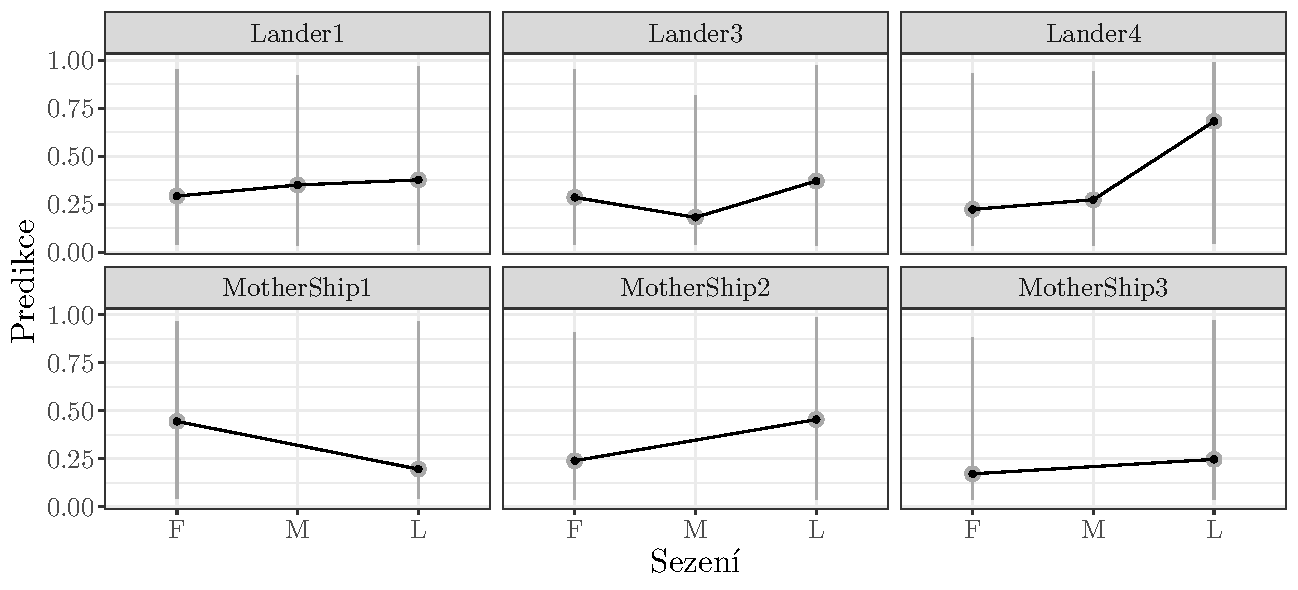
\includegraphics[width=1\linewidth]{figures/stats/hydro_test}
        \caption{Průměr, minimum a maximum (šedý rozsah) pravděpodobností
        výskytu kognitivní zátěže pro jednotlivá sezení využitím modelu
        WESAD-5s}
        \label{fig:hydro_test}
    \end{center}
\end{figure}

\begin{figure}[!htb]
    \begin{center}
        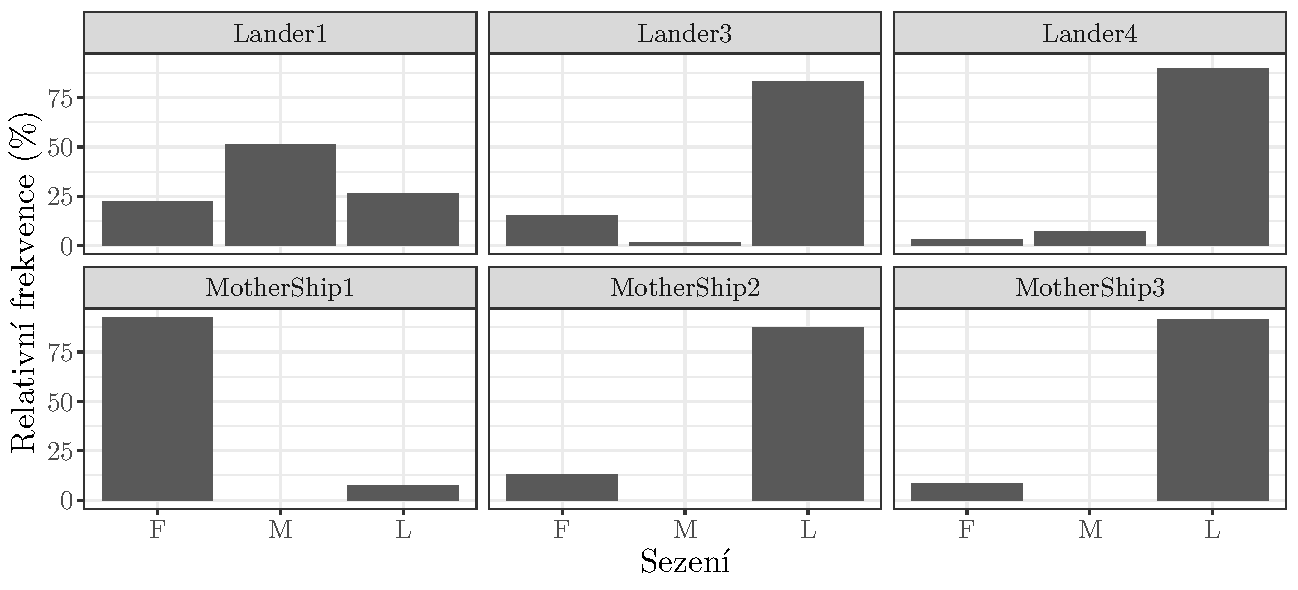
\includegraphics[width=1\linewidth]{figures/stats/hydro_test_bar}
        \caption{Relativní frekvence pravděpodobností výskytu kognitivní zátěže
        vyšších než 50~\% pro jednotlivá sezení využitím modelu WESAD-5s}
        \label{fig:hydro_test_bar}
    \end{center}
\end{figure}